\subsection{OSN 31 Методы Ньютона и секущих для решения нелинейных уравнений.}

% Рассматривается задача поиска корней нелинейного уравнения: нелинейные уравнения,
% вообще говоря, не имеют аналитического решения, поэтому для поиска решения
% используют вычислительные методы, хотя такое решение является лишь приближенным. Для конкретного итерационного метода необходимо специально выбирать
% начальное приближение, т.к. от этого выбора зависит сходимость рассматриваемых итерационных методов решения нелинейных уравнений.


\faEye \ ф-ию $f(x), ~x\in \mathbb{R}$, и ур-ие $f(x)=0.$

$\mathLet ~ x^* \in \mathbb{R}$~"--- корень уравнения, и определена его
окрестность радиуса $a$, не содержащая других корней уравнения: 
$U_a(x^*)=\{x:|x-x^*| < a\},$
причем заданная функция $f(x)$ определена на этой окрестности.
Считаем, что начальное приближение $x^0 \in U_a(x^*)$ задано.
Тогда для нахождения численного решения уравнения в
рассматриваемой окрестности необходимо построить последовательность
$\{x^n\}$, сходящуюся к~корню $x^*$ уравнения:
$\lim_{n\rightarrow\infty}f(x^n) = f(x^*) = 0.$
    
Численное решение нелинейных уравнений можно разбить на 2 этапа:
\begin{enumerate}
    \item Локализация корня, т.е. определение окрестности $U_a(x^*)$.
    \item Задание итерационного процесса~— построение последовательности
    $\{x^n\}$, сходящейся к~корню уравнения.
\end{enumerate}

\centerline{\textbf{Метод Ньютона}}

\mathLet \ в $U_a(x^*)$ существует и~не~обращается в~ноль непрерывная
первая производная функции $f(x)$: $f'(x) \neq 0,~~~x\in U_a(x^*).$

Разложим $f(x^*)$ по~формуле Тейлора в~малой окрестности точки $x\in U_a(x^*)$:
$f(x^*) =  f(x) + (x^* - x)f'(x) + \dots$, 
и отбросим в этом разложении величины, имеющие второй и выше порядок малости
по $(x^* - x)$.

Заменив $x^*$ на $x^{n+1}$ и $x$ на $x^n$, получим ур-ие 
$ f(x^n) + (x^{n + 1} - x^n)f'(x^n) = 0,~~~n\in \mathbb{Z}_+.$

Учитывая, что $f'(x^n) \neq 0$, имеем:
%
    \begin{equation}
    %
        \label{iter_proc}
        %
        x^{n + 1} = x^n - \frac{f(x^n)}{f'(x^n)},~~~n \in \mathbb{Z}_+.
    %
    \end{equation}
    %
%
Итерационный процесс поиска корня уравнения $f(x)=0$, задаваемый формулой \eqref{iter_proc},
наз-ся \textbf{итерационным методом Ньютона}.

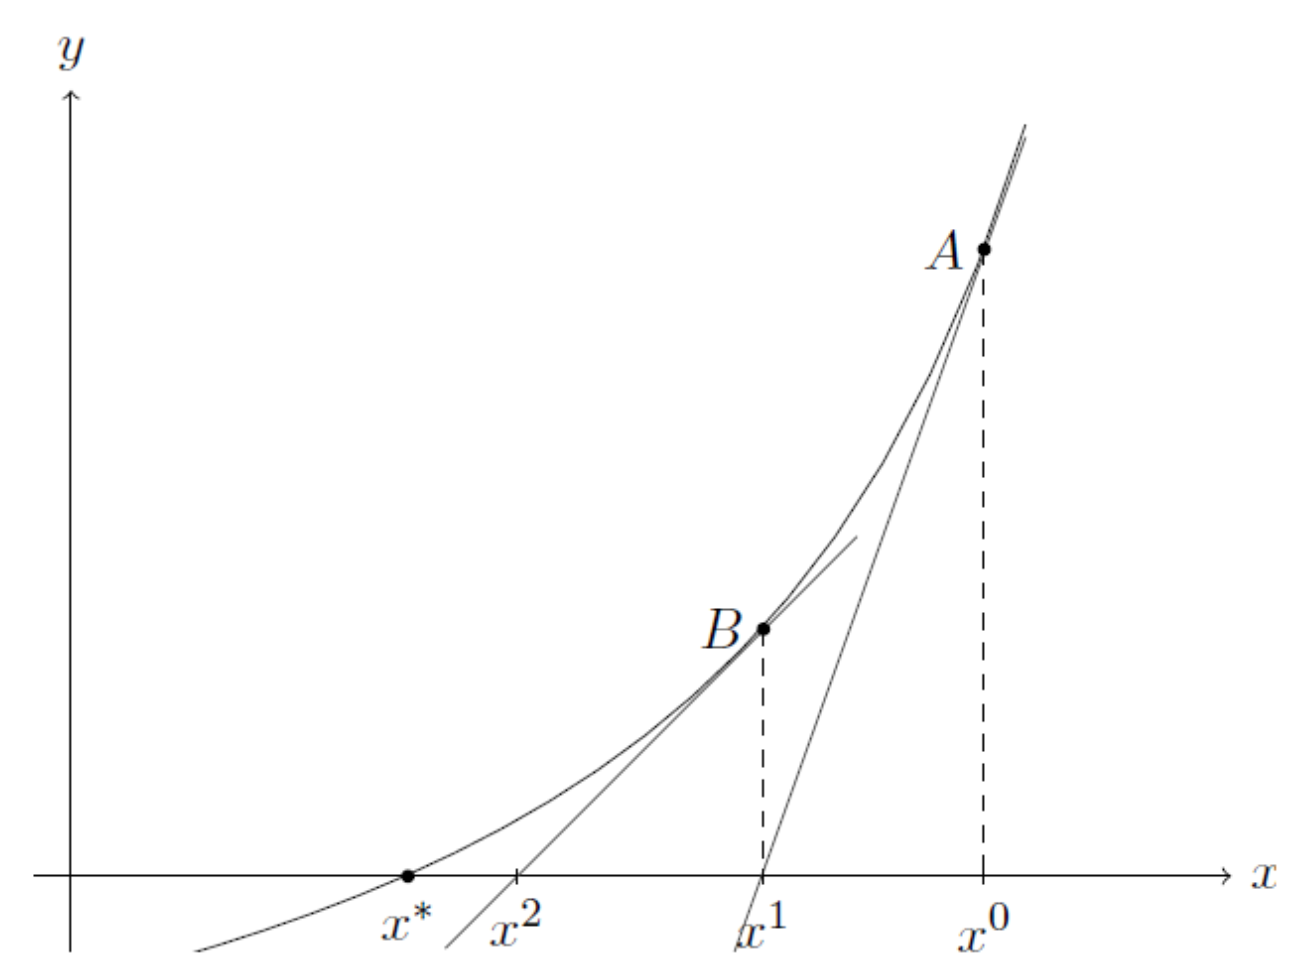
\includegraphics[scale=0.4]{pics/osn_30_0.png}

% \begin{figure}[h!]
%     \centering
%     \includegraphics[width=0.1\textwidth]{}
%     \caption{Геометрическая интерпретация метода Ньютона}
%     \label{fig:newton}
% \end{figure}
\faEye \ т. $A(x^0,f(x^0))$. Определим первую итерацию $x^1$ как абсциссу точки пересечения с осью $Ox$ касательной к $f(x)$, проведенной через т. $A$. Аналогично получаем значение $x^2$. Продолжая, на $n$-ом шаге получим значение $x^n$, приближающее корень $x^*$ уравнения $f(x)=0$ с заданной точностью.

\textbf{Зам.} При решении задач на практике часто рассматривается модифицированный
метод Ньютона, задаваемый формулой $ x^{n + 1} = x^n - \frac{f(x^n)}{f'(x^0)},~~n\in\mathbb{Z_+}$ (чтобы считать пр-ую только один раз).

\centerline{\textbf{Метод секущих}}

В методе Ньютона (\ref{iter_proc}) заменим $f'(x)$ на его дискретный аналог $\frac{f(x^n)-f(x^{n-1})}{x^n-x^{n-1}}$, получаем итерационный метод:
\begin{equation}
    x^{n+1} = x^n - \frac{(x^n - x^{n-1})f(x^n)}{f(x^n) - f(x^{n-1})}
    \label{sec}
\end{equation}
  
Итерационный процесс \ref{sec} задает двухшаговый метод решения уравнений, называемый \textbf{методом секущих}.

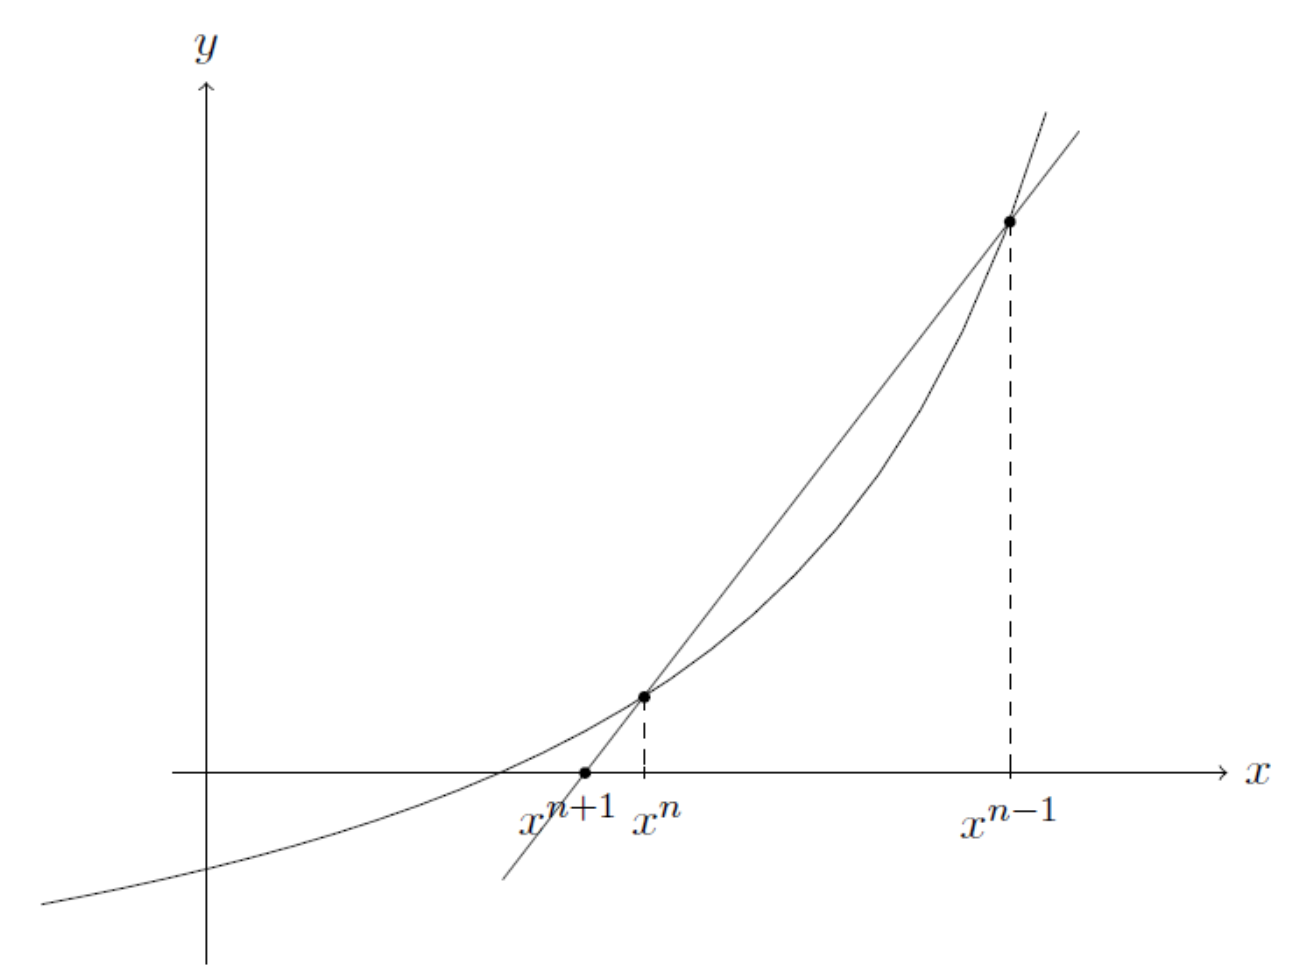
\includegraphics[scale=0.4]{pics/osn_30_1.png}

\centerline{\textbf{Сходимость метода Ньютона}}

Если рассмотреть итерационный метод Ньютона как метод простой итерации ($x^{n+1}=S(x^n), n\in \mathbb{Z_+}$) 
с функцией $S(x) = x - \frac{f(x)}{f'(x)}.$

$|S'(x)| < 1$ при $x \in U_a(x^*)$, то он сходится.
Предполагая, что функция $f(x)$ дифференцируема достаточное число раз,
продифференцируем функцию $S(x)$:
%
$$
    S'(x) = 1 - \frac{(f'(x))^2 - f(x)f''(x)}{(f'(x))^2} =
    \frac{f(x)f''(x)}{(f'(x))^2}.
$$%

\textbf{Теорема}: $\mathLet ~ \exists$ такая константа $M > 0$, для которой выполнена оценка
$\frac{1}{2}\left|S''(x)\right| \leqslant M, ~~~x \in U_a(x^*).$ 
Тогда если начальное приближение $x^0$ выбрать в соответствии с условием
$ |x^0 - x^*| < \frac{1}{M},$
то итерационный метод Ньютона сходится, и имеет место оценка:
$ |x^n - x^*| \leqslant \frac{1}{M}\left(M|x^0 - x^*|\right)^{2^n}.$

\begin{proof} Погрешность приближенного решения: $z^n = x^n - x^*.$
% Покажем, что связь между $z^n$ и $z^{n+1}$ квадратичная.

\faEye \ выражение для $z^{n+1}$:
$z^{n + 1} = x^{n + 1} - x^* = S(z^n + x^*) - S(x^*).$

Разложим $S(z^n + x^*)$ по формуле Тейлора и учитывая $S'(x^*)=0$:

$$
    z^{n + 1} = S(x^*) + S'(x^*)z^n +
    \frac{1}{2}S''(\tilde{x}^n)\left(z^n\right)^2 - S(x^*) =
    \frac{1}{2}S''(\tilde{x}^n)(z^n)^2,
$$

$$
    ~~~\tilde{x}^n=x^n+\theta z^n, ~\theta\in\mathbb{R}, ~|\theta|<1.
$$

\mathLet \ функция $f(x)$ трижды непрерывно дифференцируема в окрестности
$U_a(x^*)$. Тогда $S''(x) = \left(\frac{f(x)f''(x)}{(f'(x))^2}\right)'.$
    

$\mathLet ~ \exists$ постоянная $M > 0$ такая, что для любого $x \in U_a(x^*)$
выполняется неравенство $M \geqslant \frac{1}{2}\left|S''(x)\right|.$

Из этого неравенства и уравнения $z^{n + 1}$ следует оценка
$|z^{n+1}| \leqslant M|(z^n)^2|.$

Домножим это неравенство на $M$ и обозначим $v^n = M|z^n|$.
Тогда получим, что $v^{n+1} \leqslant (v^n)^2.$

Отсюда следует, что $v^n \leqslant (v^0)^{2^n}$, значит,
$ M|z^n| \leqslant \left(M\left|z^0\right|\right)^{2^n},$
$ |z^n| \leqslant \frac{1}{M} \left(M\left|z^0\right|\right)^{2^n}.$

Введем обозначение $q = M|z_0|$. Если $0< q < 1$,
то последовательность $\{z^n\}_{n=0}^\infty$ стремится к нулю:
$z^n \underset{n\rightarrow\infty}\longrightarrow 0,$
и итерационный метод Ньютона сходится. Условие на $q~(0<q<1)$ будет выполнено,
если $0<|z^0|<\frac{1}{M}$, то есть $|x^0 - x^*| < \frac{1}{M}$. \end{proof}

% -------- source --------
\bigbreak
[\cite[page 99-107]{chimi}]